\subsection{Algoritmo Divide et Impera}
Un algoritmo che segue la strategia \textit{divide et impera} si articola in tre fasi:
\begin{itemize}
    \item \textbf{Dividi:} Il problema è scomposto in sottoproblemi più semplici della stessa forma.
    \item \textbf{Impera:} I sottoproblemi vengono risolti ricorsivamente.
    \item \textbf{Combina:} Le soluzioni dei sottoproblemi sono combinate per ottenere la soluzione del problema originale.
\end{itemize}
La sua complessità temporale $T(n)$ è descritta da un'equazione di ricorrenza, tipicamente nella forma $T(n) = a \cdot T(n/b) + f(n)$.

\subsection{Metodi di Risoluzione delle Ricorrenze}

\subsubsection{Risoluzione Diretta Esplicita}
Consiste nello sviluppare iterativamente la ricorrenza fino a individuare un modello generale per esprimerne l'ordine di grandezza.

\subsubsection{Metodo di Sostituzione}
Consiste nel formulare un'ipotesi per la soluzione e nel verificarla rigorosamente tramite dimostrazione per induzione.

\subsubsection{Metodo dell'Albero di Ricorsione}
È una tecnica visuale per sviluppare le chiamate ricorsive e sommarne i costi livello per livello. È utile per formulare un'ipotesi di soluzione, da verificare poi con il metodo di sostituzione. Esempio di albero:
\begin{figure}[h!]
    \centering
    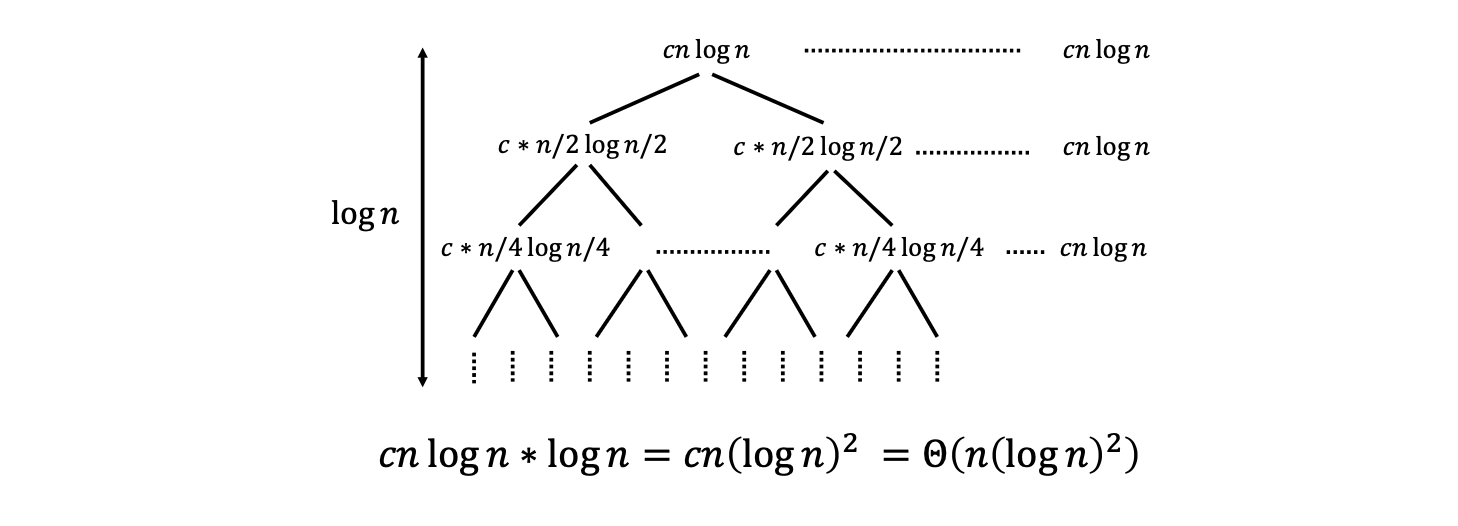
\includegraphics[width=0.8\textwidth]{images/albero_delle_ricorrenze.png}
    \caption{Esempio di un albero di ricorsione.}
    \label{fig:albero_ricorrenze}
\end{figure}

\subsubsection{Metodo per Ricorrenze Lineari}
Si applica a ricorrenze della forma $T(n) = \sum_{i=1}^{h} a_i T(n-i) + cn^k$. Posto $a := \sum a_i$, la soluzione (come limite superiore) è:
\begin{itemize}
    \item $T(n) = O(n^{k+1})$ se $a=1$.
    \item $T(n) = O(n^k a^n)$ se $a \ge 2$.
\end{itemize}

\subsubsection{Teorema Master}
Fornisce una soluzione "pronta" per ricorrenze della forma $T(n) = a \cdot T(n/b) + f(n)$ (con $a \ge 1, b > 1$). Si confronta $f(n)$ con $n^{\log_b a}$:
\begin{itemize}
    \item \textbf{Caso 1:} Se $f(n) = O(n^{\log_b a - \epsilon})$ per qualche $\epsilon > 0$, allora $T(n) = \Theta(n^{\log_b a})$.
    \item \textbf{Caso 2:} Se $f(n) = \Theta(n^{\log_b a})$, allora $T(n) = \Theta(n^{\log_b a} \log n)$.
    \item \textbf{Caso 3:} Se $f(n) = \Omega(n^{\log_b a + \epsilon})$ per qualche $\epsilon > 0$ e se $f(n)$ soddisfa una condizione di regolarità, allora $T(n) = \Theta(f(n))$.
\end{itemize}

\subsubsection*{Corollario del Teorema Master (Caso Polinomiale)}
Una versione semplificata del teorema si applica quando $f(n)$ è un polinomio della forma $\Theta(n^k)$. Data la ricorrenza $T(n) = a \cdot T(n/b) + \Theta(n^k)$:
\begin{itemize}
    \item \textbf{Caso 1:} Se $k < \log_b a$, allora $T(n) = \Theta(n^{\log_b a})$.
    \item \textbf{Caso 2:} Se $k = \log_b a$, allora $T(n) = \Theta(n^k \log n)$.
    \item \textbf{Caso 3:} Se $k > \log_b a$, allora $T(n) = \Theta(n^k)$.
\end{itemize}